\begin{tikzpicture}
    % Coordinates for the centers of the circles.
    \coordinate (C1) at (-1.3,  0.00);
    \coordinate (C2) at ( 1.3,  0.00);
    \coordinate (C3) at ( 0.0, -2.15);

    \coordinate (O)  at ( 0.0000, -0.7500);
    \coordinate (P1) at ( 0.6817, -0.2697);
    \coordinate (P2) at (-0.6817, -0.2697);
    \coordinate (P3) at ( 0.0000, -1.5198);

    % Coordinates for the labels.
    \coordinate (A) at (-1.3, 1.2);
    \coordinate (B) at ( 1.3, 1.2);
    \coordinate (C) at ( 0.0, -3.5);
    \coordinate (U) at ( 0.0, 2.5);

    % Rectangle indicating the universe set.
    \draw (-4, -4.5) rectangle (4, 3.3);

    % Fill in the intersection with cyan.
    \draw[fill=cyan, draw=none] (P1) arc(70.07:109.93:2)
                                     arc(187.8:229.50:2)
                                     arc(310.54:352.25:2);

    % Give outlines to the circles.
    \draw (C1) circle (2);
    \draw (C2) circle (2);
    \draw (C3) circle (2);

    % Labels.
    \node at (A) {$A$};
    \node at (B) {$B$};
    \node at (C) {$C$};
    \node at (U)
        {\Large{$\underset{\mathcal{U}\in\{A,B,C\}}{\bigcap}\mathcal{U}$}};
\end{tikzpicture}